\documentclass[11pt]{article}

\usepackage{abstract}
\usepackage{algorithm}
\usepackage{algorithmic}
\usepackage{amsmath}
\usepackage{amssymb}
\usepackage{bm}
\usepackage{caption}
\usepackage{CJKutf8}
\usepackage{color}
\usepackage{enumitem}
\usepackage{epsfig}
\usepackage{fancyhdr}
\usepackage{float}
\usepackage{graphics}
\usepackage{graphicx}
\usepackage{geometry}
\usepackage{indentfirst}
\usepackage{lastpage}
\usepackage{listings}
\usepackage{mathdots}
\usepackage{mathpazo}
\usepackage{multirow}
\usepackage{pstricks-add}
\usepackage{pst-blur}
\usepackage{subcaption}
\usepackage{tikz}
\usepackage{wasysym}
\usepackage{xcolor}
\usepackage[BoldFont,SlantFont,CJKsetspaces,CJKchecksingle]{xeCJK}

\allowdisplaybreaks
\DeclareMathOperator*{\argmin}{argmin}
\definecolor{Blue}{rgb}{1.,0.75,0.8}
\definecolor{mygray}{rgb}{0.5,0.5,0.5}
\definecolor{mygreen}{rgb}{0,0.6,0}
\definecolor{mymauve}{rgb}{0.58,0,0.82}
\pagestyle{empty}
\parindent 2em   %段首缩进
\setlength{\parindent}{2em}
\setCJKmainfont[BoldFont=SimHei]{SimSun}
\setCJKmonofont{SimSun}% 设置缺省中文字体
\usetikzlibrary{arrows, automata, calc, shapes}

\newcommand{\HRule}{\rule{\linewidth}{0.5mm}}
\newcommand{\hytt}[1]{\texttt{\hyphenchar\font=\defaulthyphenchar #1}}
\renewcommand{\algorithmicrequire}{\textbf{Input:}}   
\renewcommand{\algorithmicensure}{\textbf{Output:}}  
% \hyphenation{read-Sym-bol re-ad-Space-Tab-New-line str-Tab}

%\footnotesize
\lstset{ %
  backgroundcolor=\color{white},   % choose the background color; you must add \usepackage{color} or \usepackage{xcolor}
  basicstyle=\ttfamily,            % the size of the fonts that are used for the code
  breakatwhitespace=false,         % sets if automatic breaks should only happen at whitespace
  breaklines=true,                 % sets automatic line breaking
  captionpos=b,                    % sets the caption-position to bottom
  commentstyle=\ttfamily\color{mygreen},    
                                   % comment style
  deletekeywords={},               % if you want to delete keywords from the given language
  escapeinside={},                 % if you want to add LaTeX within your code
  extendedchars=true,              % lets you use non-ASCII characters; for 8-bits encodings only, does not work with UTF-8
  frame=single,                    % adds a frame around the code
  keepspaces=true,                 % keeps spaces in text, useful for keeping indentation of code (possibly needs columns=flexible)
  keywordstyle=\color{blue},       % keyword style
  language=C++,                    % the language of the code
  morekeywords={},                 % if you want to add more keywords to the set
  numbers=left,                    % where to put the line-numbers; possible values are (none, left, right)
  numbersep=5pt,                   % how far the line-numbers are from the code
  numberstyle=\tiny\color{mygray}, % the style that is used for the line-numbers
  rulecolor=\color{black},         % if not set, the frame-color may be changed on line-breaks within not-black text (e.g. comments (green here))
  showspaces=false,                % show spaces everywhere adding particular underscores; it overrides 'showstringspaces'
  showstringspaces=false,          % underline spaces within strings only
  showtabs=false,                  % show tabs within strings adding particular underscores
  stepnumber=1,                    % the step between two line-numbers. If it's 1, each line will be numbered
  stringstyle=\color{mymauve},     % string literal style
  tabsize=2,                       % sets default tabsize to 2 spaces
  title=\lstname                   % show the filename of files included with \lstinputlisting; also try caption instead of title
}

\pagestyle{fancy}
\rhead{page \thepage\ of \pageref{LastPage}}
%\chead{}
\lhead{操作系统实验报告}
\cfoot{}

\begin{document}

\title{操作系统实验4 \quad 进程的管道通信}
\author{计算机1202 \quad 张艺瀚\\学号:20123852}
\maketitle

\thispagestyle{fancy}
%\newpage
\normalsize 

% 题目、目的、要求
% 修改后的程序流程图
% 调试正确的源程序
% 运行结果及说明
% 回答问题:
% 进程间的互斥表现在哪里?
% 进程间的同步表现在哪里?
% 你的程序采用什么方法实现上述关系?

\section{实验题目}
编程实现进程的管道通信程序

\section{实验目的}
这是一个验证型实验。通过对给出的程序进行验证、修改,进一步加深理解进程的概念,了解同步和通信的过程,掌握进程通信和同步的机制,特别是利用缓冲区进行同步和通信的过程。通过补充新功能,加强对知识的灵活运用,培养创新能力。

\section{实验要求}
\begin{enumerate}
\item 加深对进程概念的理解,明确进程和程序的区别;
\item 学习进程创建的过程,进一步认识并发执行的实质;
\item 分析进程争用资源的现象,学习解决进程互斥的方法;
\item 学习解决进程同步的方法;
\item 掌握Linux系统进程间通过管道通信的具体实现方法。
\end{enumerate}

\section{程序流程图}
见图\ref{fig: main}

\tikzstyle{startstop} = [rectangle, rounded corners, minimum width=2cm, minimum height=1cm,text centered, draw=black, fill=red!30]
\tikzstyle{io} = [trapezium, trapezium left angle=70, trapezium right angle=110, minimum width=2cm, minimum height=1cm, text centered, draw=black, fill=blue!30]
\tikzstyle{operation} = [rectangle, minimum width=2cm, minimum height=1cm, text centered, draw=black, fill=orange!30]
\tikzstyle{judge} = [diamond, minimum width=2cm, minimum height=1cm, text centered, draw=black, fill=green!30]
\tikzstyle{arrow} = [thick,->,>=stealth]

\begin{figure}[htbp]
\centering
\begin{tikzpicture}[node distance=2cm]
%定义流程图具体形状
\node (a) [startstop] at(0,1)      {开始};
\node (b) [operation] at(0,-0.5)      {创建管道};
\node (c) [operation] at(0,-2)      {创建子进程1};
\node (d) [judge] at(0,-5)      {\begin{tabular}{c} 子进程1 \\ 被调度? \end{tabular}};
\node (e) [operation] at(0,-7 - 1)      {锁管道};
\node (f) [operation] at(0,-8.5 - 1)      {写消息1};
\node (g) [operation] at(0,-10 - 1)      {解锁};
\node (h) [operation] at(0,-11.5 - 1)      {子进程1结束};

\node (i) [operation] at(5,-2)      {创建子进程2};
\node (j) [judge] at(5,-5)      {\begin{tabular}{c} 子进程2 \\ 被调度? \end{tabular}};
\node (k) [operation] at(5,-7 - 1)      {锁管道};
\node (l) [operation] at(5,-8.5 - 1)      {写消息2};
\node (m) [operation] at(5,-10 - 1)      {解锁};
\node (n) [operation] at(5,-11.5 - 1)      {子进程2结束};

\node (o) [operation] at(10,-8)      {等待子进程1执行完};
\node (p) [operation] at(10,-9.5)      {读消息1};
\node (q) [operation] at(10,-11)      {等待子进程2执行完};
\node (r) [operation] at(10,-12.5)      {读消息2};
\node (s) [startstop] at(10,-14)      {结束};

%连接具体形状
\draw [arrow](a) -- (b);
\draw [arrow](b) -- (c);
\draw [arrow](c) -- (d);
\draw [arrow](d) -- node[anchor=east] {Y} (0, -7) -- (e);
\draw [arrow](d) -- node[anchor=south] {N} (-3, -5) -- (-3, -13.5) -- (0, -13.5);
\draw [arrow](e) -- (f);
\draw [arrow](f) -- (g);
\draw [arrow](g) -- (h);

\draw [arrow](h) -- (0, -13.5) -- (2, -13.5) -- (2, -1) -- (5, -1) -- (i);

\draw [arrow](i) -- (j);
\draw [arrow](j) -- node[anchor=east] {Y} (5, -7) -- (k);
\draw [arrow](j) -- node[anchor=south] {N} (3, -5) -- (3, -13.5) -- (5, -13.5);
\draw [arrow](k) -- (l);
\draw [arrow](l) -- (m);
\draw [arrow](m) -- (n);

\draw [arrow](n) -- (5, -13.5) -- (7.5, -13.5) -- (7.5, -7) -- (10, -7) -- (o);

\draw [arrow](o) -- (p);
\draw [arrow](p) -- (q);
\draw [arrow](q) -- (r);
\draw [arrow](r) -- (s);

%\draw [arrow]( ) -- node[anchor=east] {是} ( );
%\draw [arrow]( ) -- node[anchor=south] {否} ( );
\end{tikzpicture}
\caption{主过程}
\label{fig: main}
\end{figure}

\section{源程序}
\begin{lstlisting}[caption = {代码清单}, label = {lst: code}]
#include <errno.h>
#include <stdio.h>
#include <stdlib.h>
#include <sys/types.h>
#include <sys/wait.h>
#include <unistd.h>
int main()
{
  pid_t pc1, pc2, pr1, pr2;
  int fd[2];
  char buf1[50], buf2[50], s[50];
  pipe(fd);
  while((pc1 = fork()) == -1);
  if(pc1 < 0){
    printf("create child process1 error: %s\n", strerror(errno));
    exit(1);
  }else if(pc1 == 0){
    lockf(fd[1], 1, 0);
    sprintf(buf1, "child process1 %d is sending a msg", getpid());
    write(fd[1], buf1, 50);
    printf("in process1 %d, sending a msg\n", getpid());
    lockf(fd[1], 0, 0);
    exit(0);
  }
  while((pc2 = fork()) == -1);
  if(pc2 < 0){
    printf("create child process2 error: %s\n", strerror(errno));
    exit(1);
  }else if(pc2 == 0){
    lockf(fd[1], 1, 0);
    sprintf(buf2, "child process2 %d is sending a msg", getpid());
    write(fd[1], buf2, 50);
    printf("in process2 %d, sending a msg\n", getpid());
    lockf(fd[1], 0, 0);
    exit(0);
  }
  printf("in parent process %d\n", getpid());
  pr1 = wait(0);
  if(pr1 > 0){
    read(fd[0], s, 50);
    printf("parent process %d received a msg: %s\n", getpid(), s);;
  }else{
    printf("error: %s\n", strerror(errno));
  }
  pr2 = wait(0);
  if(pr2 > 0){
    read(fd[0], s, 50);
    printf("parent process %d received a msg: %s\n", getpid(), s);
  }else{
    printf("error: %s\n", strerror(errno));
  }
  return 0;
}
\end{lstlisting}

\section{运行结果及其说明}
运行结果见图\ref{fig: pipe}。两个子进程互斥使用管道,父子进程之间同步传递消息。子进程的调度顺序随机,不受用户控制,有时会出现子进程2先于子进程1调度的情况。

\begin{center}
\begin{figure}[htbp]
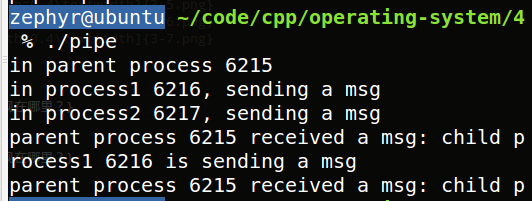
\includegraphics[width=\textwidth]{pipe.png}
\caption{运行结果}
\label{fig: pipe}
\end{figure}
\end{center}

\section{回答问题}
\subsection{进程间的互斥表现在哪里?}
两个子进程都要对管道写消息,管道作为两个子进程共享的资源,应当互斥使用,每个子进程使用时要做互斥保护(使用前加锁,使用后解锁)。

\subsection{进程间的同步表现在哪里?}
父子进程之间传递消息,只有子进程写入后,父进程才能读出,父进程读子进程i的消息前要先等待子进程i执行完毕。

\subsection{你的程序采用什么方法实现上述关系?}
互斥:子进程写消息前使用lockf对管道加锁,写后用lockf解锁;同步:子进程结束后exit表执行完毕,父进程读消息前wait对应子进程。使用fork的返回值区分父进程和两个字进程的代码模块。

\end{document}
